\section{Execution Plan Generation}
\label{sec:queryPro}

Our runtime execution of \Dlog programs differs from the traditional
implementation patterns for both network protocols and database
queries.  Network protocol implementations often center around local
state machines that emit messages, triggering state transitions at
other state machines.  By contrast, the runtime systems we have built
for \Dlog and \Overlog are distributed dataflow execution engines,
similar in spirit to those developed for parallel database systems,
and echoed in recent parallel map-reduce~\cite{mapreduce} implementations.
\jmh{We could lose the MapReduce citation to make room for something more interesting.}
Set-oriented operators are replicated on each node in the network,
with the dataflows between the operators partitioned and shuffled by
value across nodes. However, the recursion in  Datalog introduces
cycles into these dataflows. The combination of recursive flows and
the asynchronous communication inherent in wide-area systems presents
new challenges that we had to overcome.

In this section we describe the steps required to automatically generate a distributed dataflow execution
plan from a \Dlog program. We first focus on generating an execution
plan in a centralized implementation, before extending the techniques
to the network scenario.

\subsection{Centralized Plan Generation}
\label{sec:semiNaive}

In generating the centralized plan, we utilize the well-known {\em
semi-\naive fixpoint}~\cite{semi,semi1} evaluation mechanism that
ensures no redundant evaluations. As a quick review, in semi-\naive
(SN) evaluation, input tuples computed in the previous iteration of a
recursive rule execution are used as input in the current iteration to
compute new tuples. Any new tuples that are generated for the first
time in the current iteration are then used as input to the next
iteration. This is repeated until a fixpoint is achieved (i.e., no new
tuples are produced).

The semi-\naive rewritten rule for rule \nd{sp2} is shown below:

\begin{NDlog}
sp2-1 delta_path_new(@Src,Dest,Nxt,Path,Cost) :- \link(@Src,Nxt,C1),
          delta_path_old(@Nxt,Dest,Nxt2,P2,C2), 
          Cost = C1 + C2, 
          Path = f\_concatPath(Nxt,P2).
\end{NDlog}

\begin{figure*}[ht]
\centering
%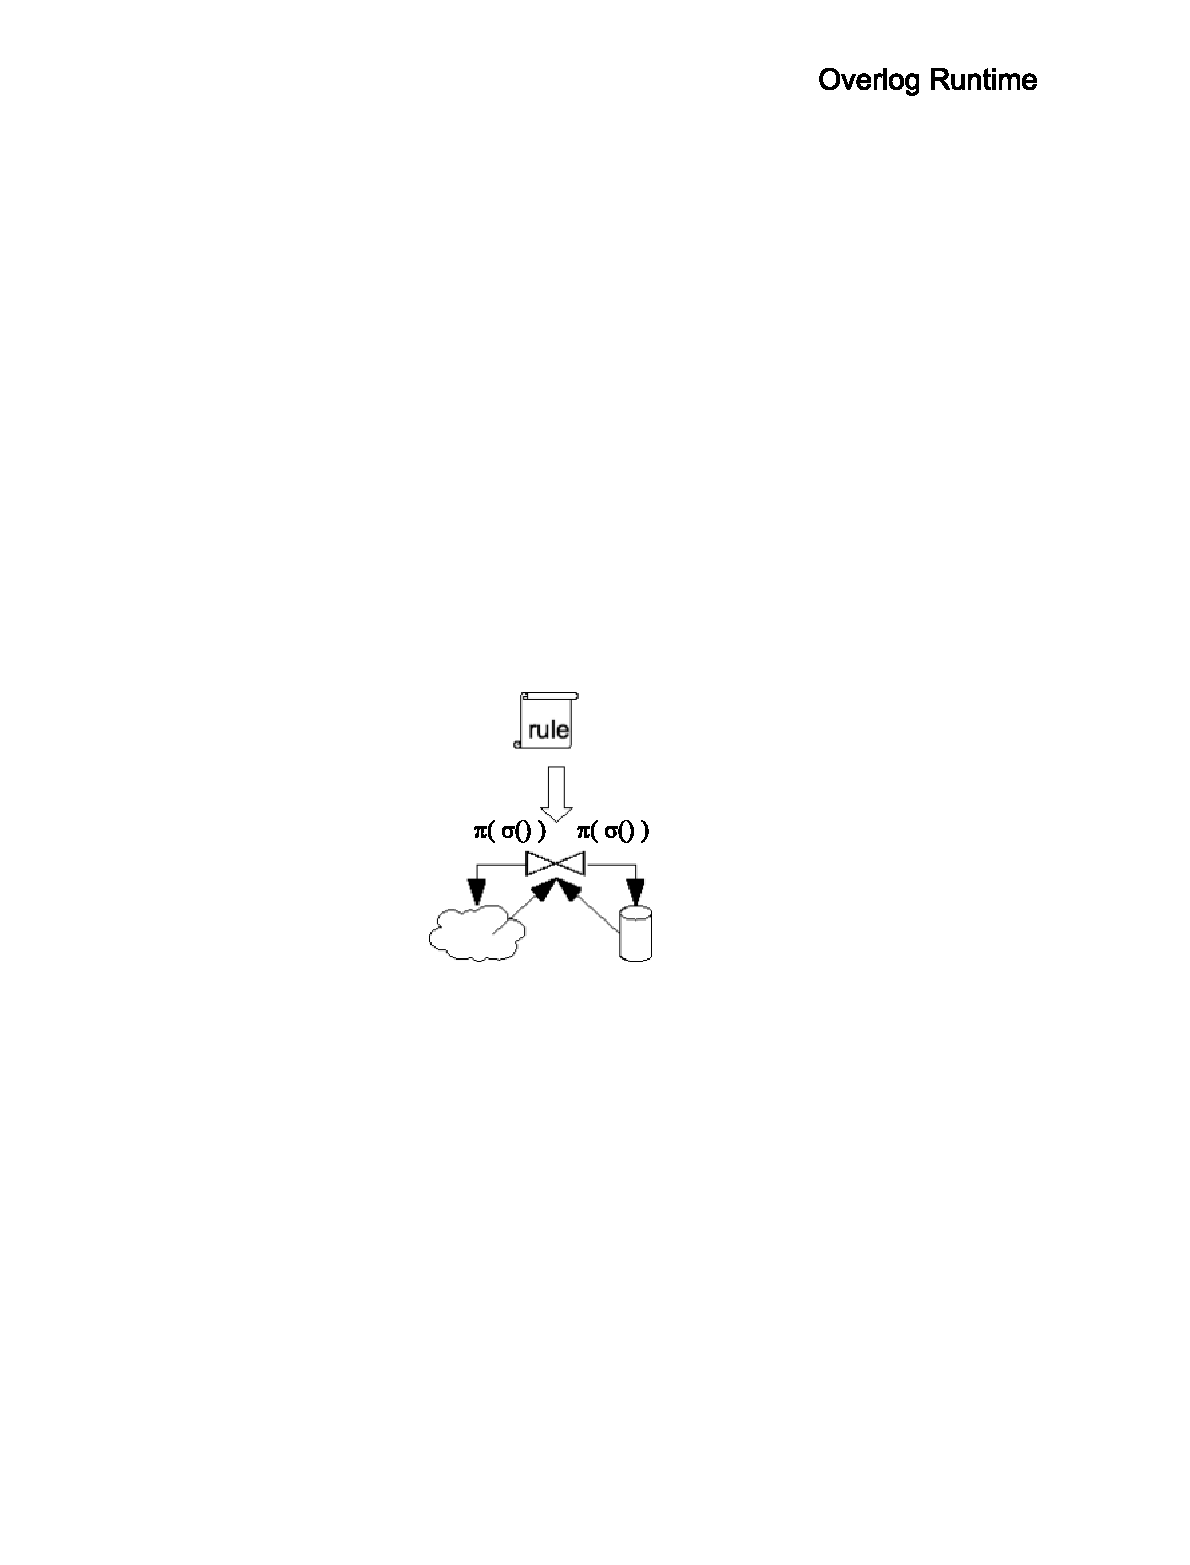
\epsfig{file=images/dataflow.eps, width=5in}
  
\includegraphics[width=5in]{graphs/dataflow}
\caption{\label{Dataflow}{\small Rule strand for rule SP2-1 in
    \Sys. Output paths that are generated from the strand are ``wrapped
    back'' as input into the same strand. }}
\end{figure*}                                        


Figure~\ref{Dataflow} shows the dataflow realization for rule \nd{sp2-1}
using the conventions of \Sys. We will briefly explain how the
semi-\naive evaluation is achieved here. Each semi-\naive rule is
implemented as a {\em rule strand}. Each strand consists of a number
of relational operators. The example strand receives new
\nd{delta\_path\_old} tuples generated in the previous iteration to
generate new paths (\nd{delta\_path\_new}) which are then inserted
into the \nd{path} table (with duplicate elimination) for further
processing in the next iteration.


In Algorithm~\ref{alg:sn}, we show the pseudocode for a centralized
\Sys implementation of multiple semi-\naive rule strands where each
rule has the form 

\begin{NDlog}
delta_p^new_j :- p^old\_1, ...,  p^old\_k-1, delta^p\_old\_k,
                 p\_k+1, ..., p\_n, b\_1, b\_2,...,b\_m;
\end{NDlog}  
\nd{p\_1, ..., p\_n} are recursive predicates and
\nd{b\_1, .... b\_m} are base predicates. \nd{delta\_p\_old\_k} refers
to \nd{p\_k} tuples generated for the first time in the previous
iteration. \nd{p\_old\_k} refers to all \nd{p\_k} tuples generated before
the previous iteration.  These rules are logically equivalent to
rules of the form 
\begin{NDlog}
delta_p^new_j :- p_1, ...,  p_k-1, delta\_p^old\_k,
                 p\_k+1, ..., p\_n, b\_1, b\_2,...,b\_m;
\end{NDlog}  
but have the advantage of avoiding redundant inferences within each
iteration.

\jmh{I could not manage to get a mix of NDLog formatting and math mode for triangles and super/sub-scripts.  Help?}


\vspace{2pt}
\begin{Algorithm}[ht]
  \begin{programbox}
%    |Initialize all | p_{i} | and | \triangle p^{new}_{i} to | null |
    \WHILE \exists B_{k}.size > 0
     \forall B_{k} | where | B_{k}.size > 0, \triangle p^{old}_{k} \leftarrow B_{k}.flush()
	|execute all rule strands | 	
	\FOREACH | recursive predicate | p_{j} 
	  p^{old}_{j} \leftarrow p^{old}_{j} \union \triangle p^{old}_{j}
	  B_{j} \leftarrow \triangle p^{new}_{j} - p^{old}_{j}
	  p_{j} \leftarrow p^{old}_{j} \union B_{j}
	  \triangle p^{new}_{j} \leftarrow \emptyset
%	\END
%    \END	      
\end{programbox}
\caption{Semi-\naive (SN) Evaluation in \Sys}
\label{alg:sn}
\end{Algorithm}
%end{boxedminipage}
\vspace{2pt}


In the algorithm, $B_{k}$ denotes the buffer for $p_{k}$ tuples
generated in the previous iteration
($\triangle$$p^{old}_{k}$). Initially, $p_{k}$, $p^{old}_{k}$,
$\triangle$$p^{old}_{k}$ and $\triangle$$p^{new}_{k}$ are empty. As a
base case, we execute all the rules to generate the initial $p_{k}$
tuples, which are inserted into the corresponding $B_{k}$ buffers.
Each subsequent iteration of the while loop consists of flushing all
existing $\triangle$$p^{old}_{k}$ tuples from $B_{k}$ and executing
all rule strands to generate $\triangle$$p^{new}_{j}$ tuples, which
are used to update $p^{old}_{j}$, $B_{j}$ and $p_{j}$
accordingly. Note that only new $p_{j}$ tuples generated in the
current iteration are inserted into $B_{j}$ for use in the next
iteration. Fixpoint is reached when all buffers are empty.

 
\subsection{Distributed Plan Generation}
\label{subsec:ruleLocalization}

In the distributed implementation of the path-vector program,
non-local rules whose body predicates have different location
specifiers cannot be executed at a single node, since the tuples that
must be joined are situated at different nodes in the network. A {\em
  rule localization} rewrite step ensures that all tuples to be joined
are at the same node. This allows a rule body to be locally
computable.


\begin{figure}[ht]
\centering
  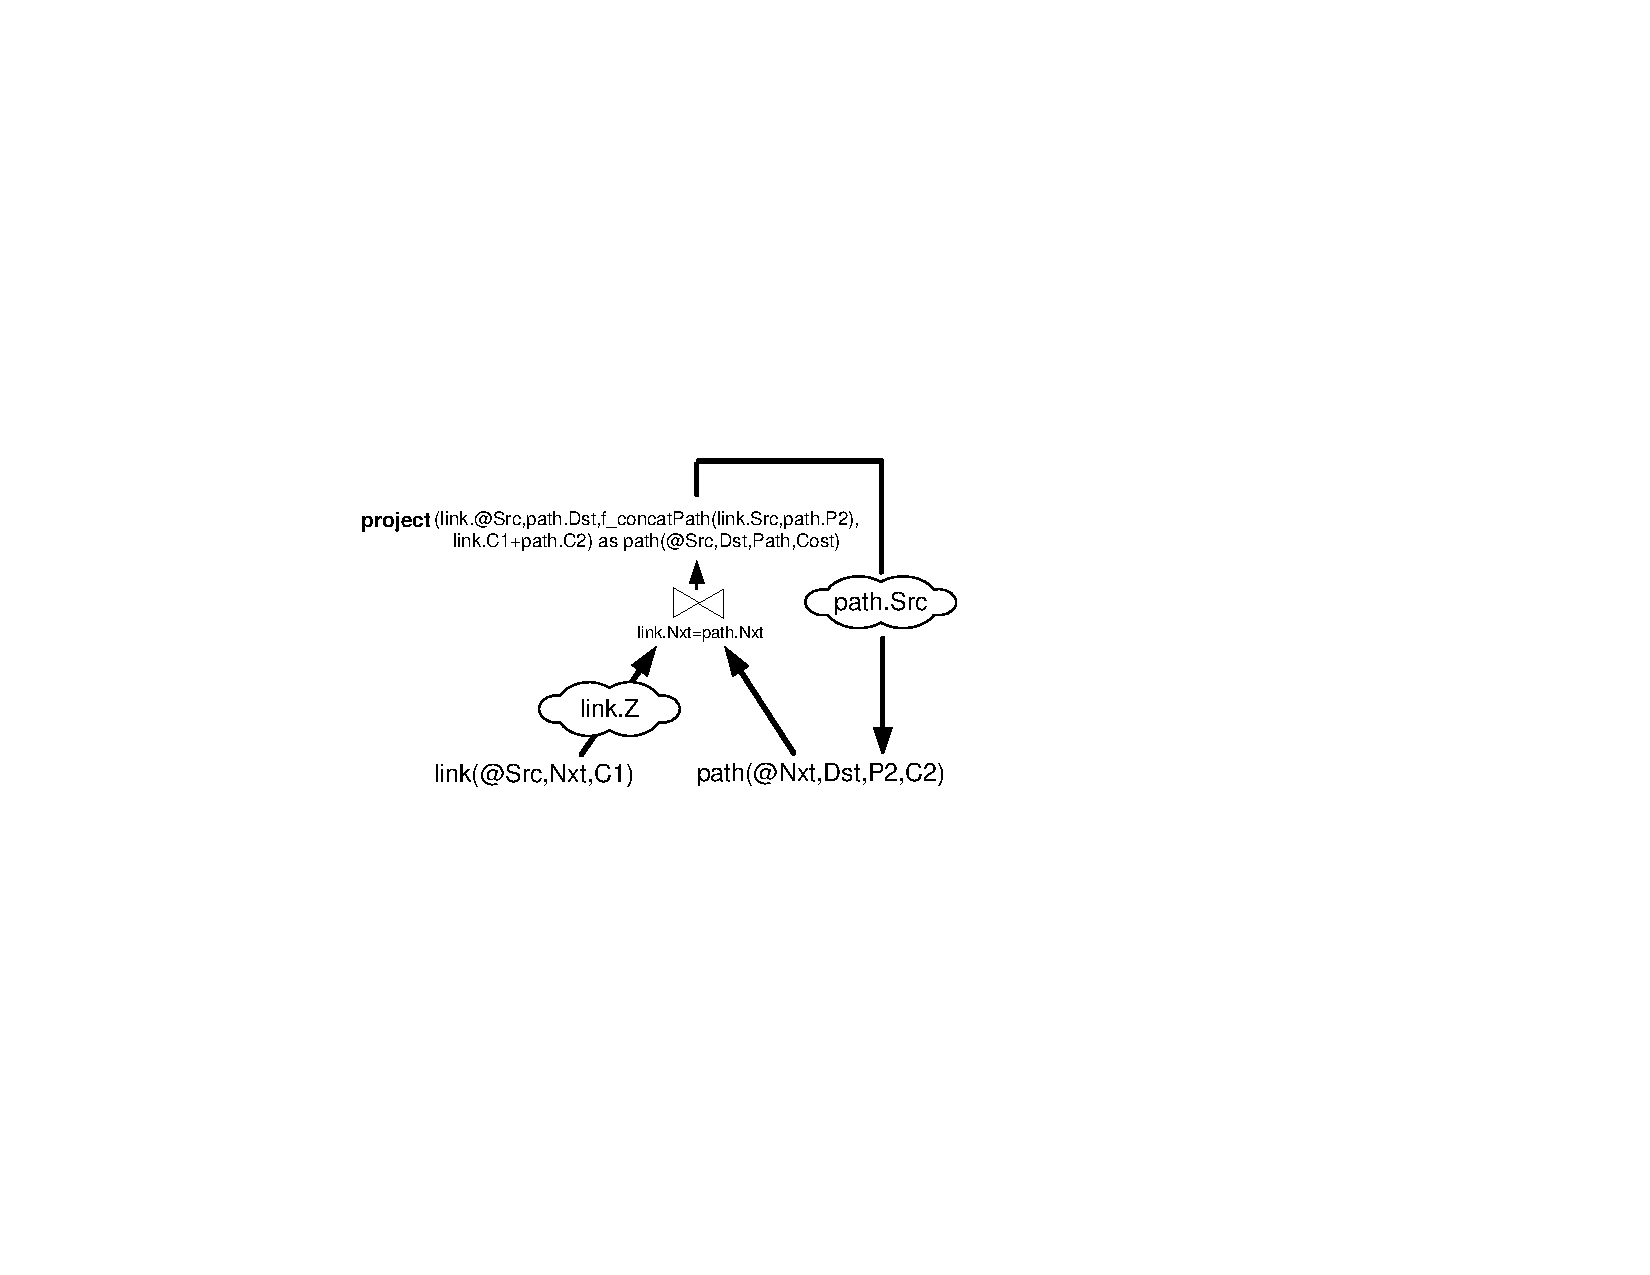
\includegraphics[width=2.5in]{graphs/reachable}
%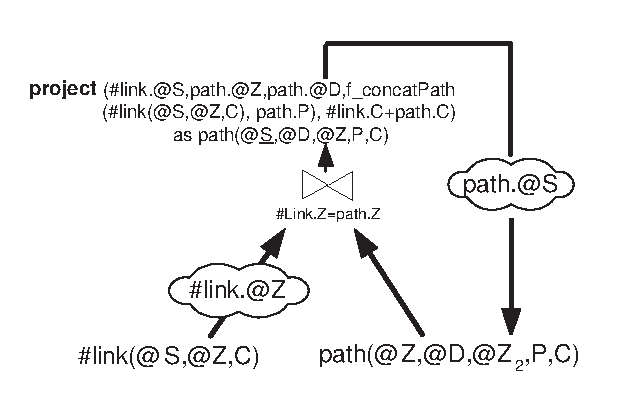
\includegraphics[width=2.5in]{images/reachable.eps}
\caption{\label{Right Reachable}\emph{\small Logical Query Plan for rule
    SP2. }}
\end{figure}                                              


Consider the rule \nd{sp2} from the path-vector program, where the \nd{link} and
\nd{path} predicates have different location specifiers. These two
predicates are joined by a common \nd{@Nxt} address
field. Figure~\ref{Right Reachable} shows the corresponding logical
query plan depicting the distributed join. The clouds represent an
``exchange''-like operator~\cite{volcano} that forwards tuples from
one network node to another; clouds are labeled with the \nd{link}
attribute that determines the tuple's recipient. The first cloud
(\nd{link.@Nxt}) sends \nd{link} tuples to the neighbor nodes indicated by their
destination address fields, in order to join with matching \nd{path} tuples
stored by their source address fields. The second cloud (\nd{path.@Src})
transmits for further processing new \nd{path} tuples computed from the
join, setting the recipient according to the source address field.

Based on the above distributed join, rule \nd{sp2} can be rewritten into
the following two rules. Note that all predicates in the body of \nd{sp2a}
have the same location specifiers; the same is true of \nd{sp2b}.

\begin{NDlog}
sp2a  linkD(@Nxt,Src,C) :- link(@Src,Nxt,C).
sp2b  path(@Src,Dest,Nxt,P,C) :- linkD(@Nxt,Src,C1), 
          path(@Nxt,Dest,Nxt2,P2,C2), C = C1 + C2,                               
          P = f_concatPath(Nxt,P2).
\end{NDlog}


\begin{figure*}[ht]
\centering
  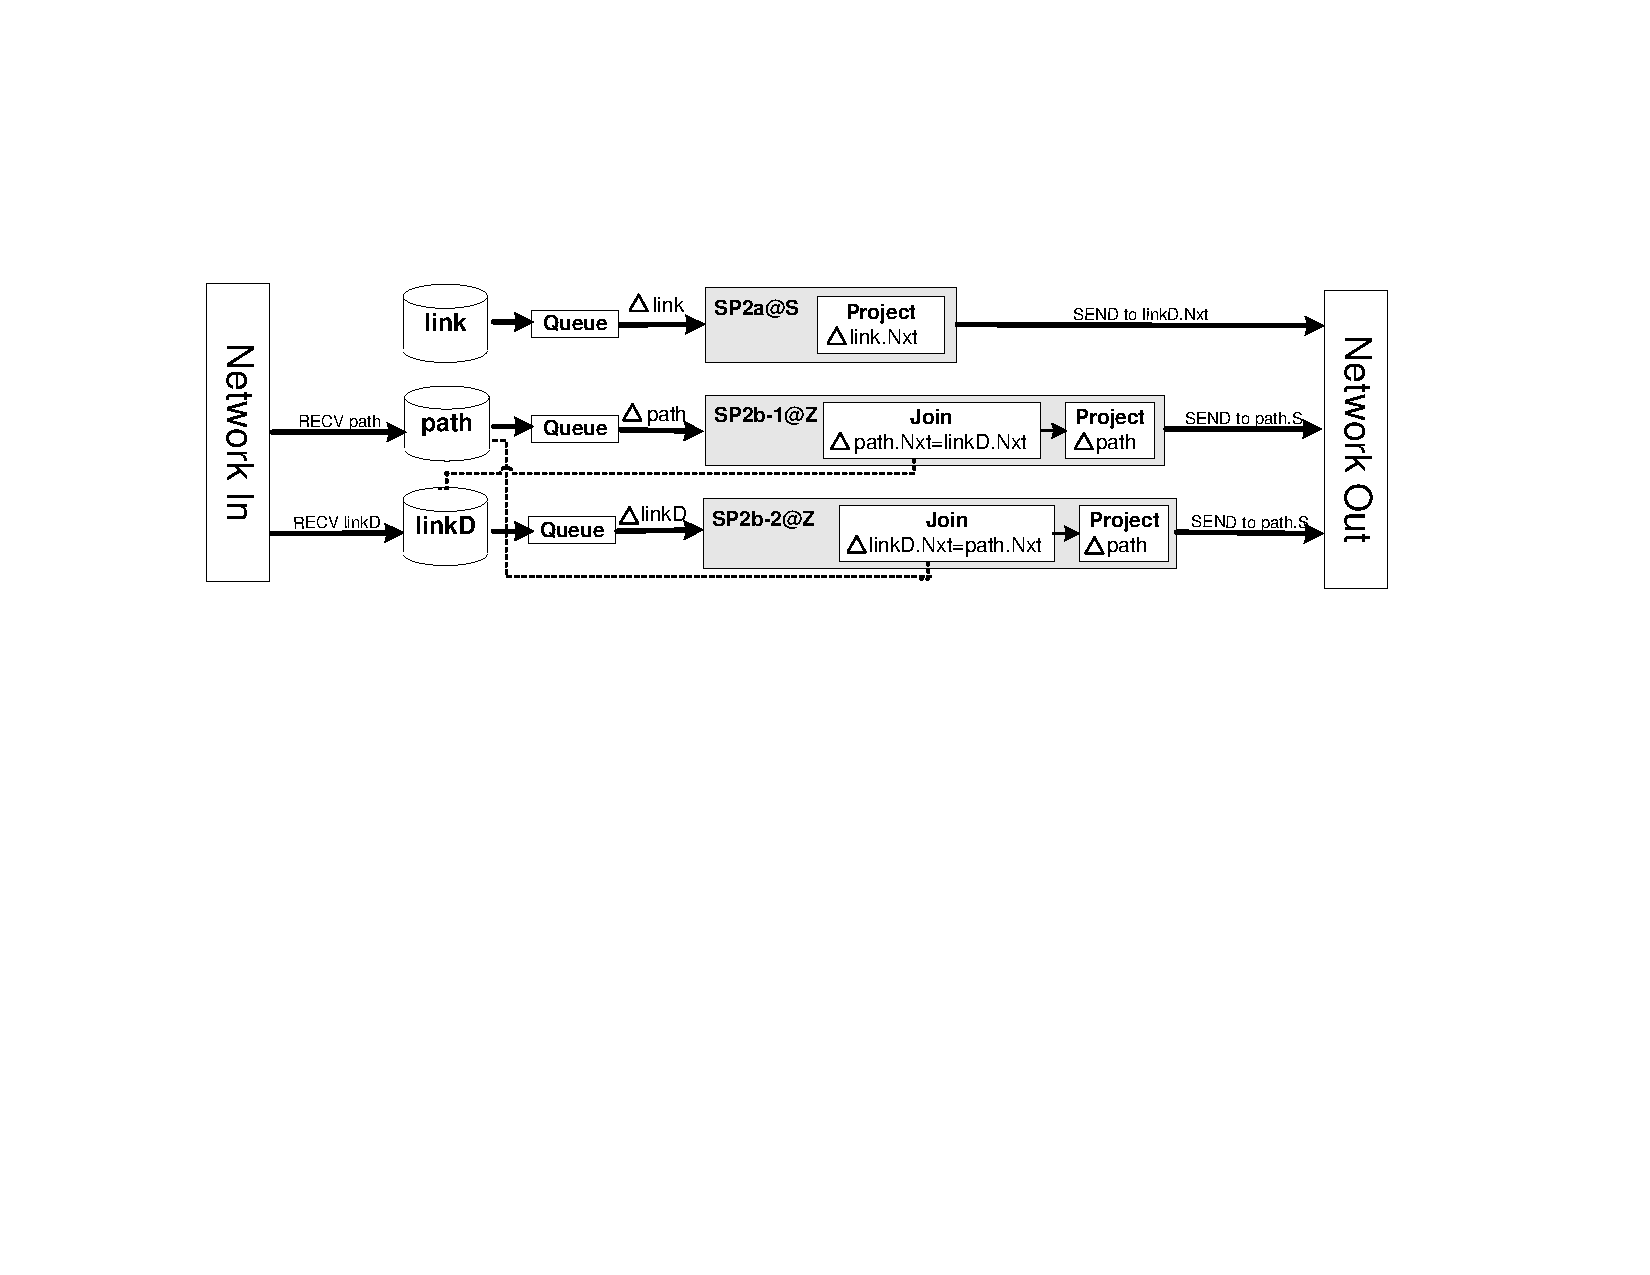
\includegraphics[width=5in]{graphs/dataflow1.pdf}
%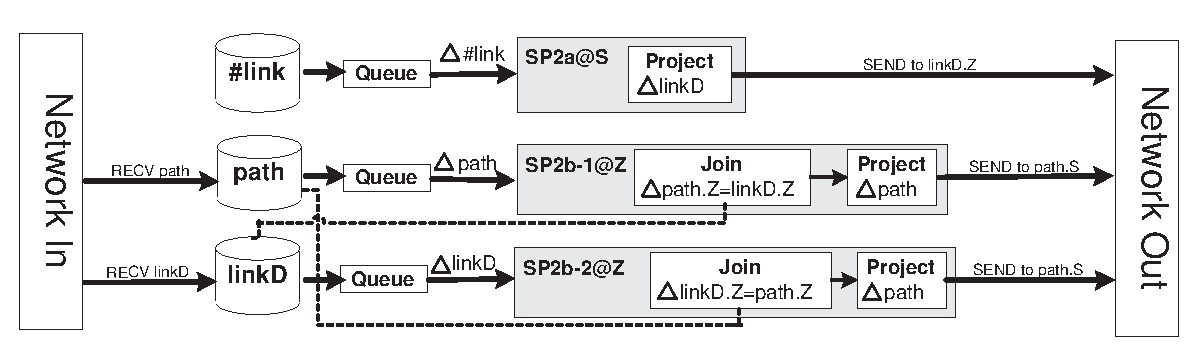
\epsfig{file=graphs/dataflow1.eps, width=5in}
\caption{\label{Dataflow1}{\small Rule strands for the distributed
    version of SP2 after localization in \Sys. }}
\end{figure*}                                        

The rewrite is achievable because the \nd{link} and \nd{path} predicates,
although at different locations, share a common join address
field. The details of the rewrite algorithm and associated proofs are
described in a longer article~\cite{declareNetworks}.

Returning to our example, after rule localization we perform the 
semi-\naive rewrite, and then generate the rule strands shown in
Figure~\ref{Dataflow1}.  Unlike the centralized strand in
Figure~\ref{Dataflow}, there are now three rule strands. The extra two
strands (\nd{SP2a@Src} and \nd{SP2b-2@Nxt}) are used as follows. Rule strand
\nd{SP2a@Src} sends all existing links to the destination address field
as \nd{linkD} tuples.  Rule strand \nd{SP2b-2@Nxt} takes the new \nd{linkD}
tuples it received via the network and performs a join operation with
the local \nd{path} table to generate new paths.


\subsection{Relaxing Semi-\naive Evaluation}
\label{sec:psn}
In our distributed implementation, the execution of rule strands can
depend on tuples arriving via the network, and can also result in new
tuples being sent over the network. Traditional semi-\naive evaluation
completely evaluates all rules on a given set of facts, i.e., completes
the {\em iteration}, before considering any new facts.  In a
distributed execution environment where messages can be delayed or
lost, the completion of an iteration in the traditional sense can only
be detected by a consensus computation across multiple nodes, which is
expensive; further, the requirement that many nodes complete the
iteration together (a ``barrier synchronization'' in parallel
computing terminology) limits parallelism significantly by restricting
the rate of progress to that of the slowest node.

We address this by making the notion of iteration local to a node.
New facts might be generated through local rule execution, or might be
received from another node while a local iteration is in progress.  We
propose and prove correct a variation of semi-\naive iteration called
{\em pipelined semi-naive} (PSN) to handle this situation.  PSN
extends SN to work in an asynchronous distributed setting. PSN relaxes
semi-\naive evaluation to the extreme of processing each tuple as it
is received. This provides opportunities for additional optimizations
on a per-tuple basis, at the potential cost of set-oriented local
processing. New tuples that are generated from the semi-\naive rules,
as well as tuples received from other nodes, are used immediately to
compute new tuples without waiting for the current (local) iteration
to complete.


\vspace{2pt}
%begin{boxedminipage}{3in}
\begin{Algorithm}[ht]
  \begin{programbox}
    \WHILE \exists Q_{k}.size > 0
     t^{old,i}_{k} \LAR Q_{k}.dequeueTuple()
     \FOREACH | rule strand execution | 
     |\quad | \triangle p^{new,i+1}_{j} :- p_{1},..,p_{k-1},t^{old,i}_{k},p_{k+1},..,p_{n},b_{1},b_{2},...,b_{m}
       |\quad| \FOREACH  t^{new,i+1}_{j} \in \triangle p^{new,i+1}_{j}
         \IF t^{new,i+1}_{j} \notin p_{j} 
	 \THEN p_{j} \leftarrow p_{j} \union t^{new,i+1}_{j}
 	      Q_{j}.enqueueTuple(t^{new,i+1}_{j})
%	 \FI
%     \END      
%     \END
%   \END
\end{programbox}
\caption{Pipelined Semi-\naive (PSN) Evaluation}
\label{alg:psn}
\end{Algorithm}
%end{boxedminipage}
\vspace{2pt}


Algorithm~\ref{alg:psn} shows the pseudocode for PSN. Each tuple,
denoted $t$, has a superscript ($old$/$new$, $i$) where $i$ is its
corresponding iteration number in SN evaluation. Each processing step
in PSN consists of dequeuing a tuple $t^{old,i}_{k}$ from $Q_{k}$ and
then using it as input into all corresponding rule strands. Each
resulting $t^{new,i+1}_{j}$ tuple is pipelined, stored in its
respective $p_{j}$ table (if a copy is not already there), and
enqueued into $Q_{j}$ for further processing. Note that in a
distributed implementation, $Q_{j}$ can be a queue on another node,
and the node that receives the new tuple can immediately process the
tuple after the enqueue into $Q_{j}$. For example, the dataflow in
Figure~\ref{Dataflow1} is based on a distributed implementation of
PSN, where incoming \nd{path} and \nd{linkD} tuples received via the network
are stored locally, and enqueued for processing in the corresponding
rule strands.

To fully pipeline evaluation, we have also removed the distinctions
between $p^{old}_{j}$ and $p_{j}$ in the rules. Instead, a timestamp
(or monotonically increasing sequence number) is added to each tuple
at arrival, and the join operator matches each tuple only with tuples
that have the same or older timestamp. This allows processing of
tuples immediately upon arrival, and is natural for network message
handling. This represents an alternative ``book-keeping'' strategy to
the rewriting used in SN to ensure no repeated inferences. Note that
the timestamp only needs to be assigned locally, since all the rules
are localized.

%While PSN enables fully pipeline evaluation, it is worth noting that PSN
%can allow just as much buffering as BSN with the additional flexibility
%of full pipelining.

We prove elsewhere~\cite{declareNetworks} that PSN generates the same
results as SN and does not repeat any inferences, as long as the \Dlog
program is monotonic and network messages between two network nodes are
delivered in FIFO order. 
% \reminder{Briefly describe processing of soft-state
  % events and data.}



\subsection{Incremental Maintenance}

In practice, most network protocols are executed over a long period of
time, and the protocol incrementally updates and repairs routing
tables as the underlying network changes (link failures, node
departures, etc.).  To better map into practical networking scenarios,
one key distinction that differentiates the execution of \Dlog from
earlier work in Datalog is our support for continuous rule execution
and results materialization, where all tuples derived from \Dlog rules
are materialized and incrementally updated as the underlying network
changes. As in network protocols, such incremental maintenance is
required both for timely updates and for avoiding the overhead of
recomputing all routing tables ``from scratch'' whenever there are
changes to the underlying network. In the presence of insertions and
deletions to base tuples, our original incremental view maintenance
implementation utilizes the count algorithm~\cite{viewincremental} to
ensure that deletions only tuples that no longer are derivable. This
has subsequently been improved in ~\cite{absorption} via the use of a
compact form of data provenance encoded using binary decision diagrams
shipped with each derived tuple.

In general, updates could occur very frequently, at a period that is
shorter than the expected time for a typical query to reach a
fixpoint.  In that case, query results can never fully reflect the
state of the network. We focus our analysis instead on a {\em bursty}
model. In this weaker, but still fairly realistic model, updates are
allowed to happen during query processing.  However, we make the
assumption that after a burst of updates, the network eventually {\em
  quiesces} (does not change) for a time long enough to allow all the
queries in the system to reach a fixpoint.  Unlike the continuous
model, the bursty model is amenable to simpler analysis; our results
on that model provide some intuition as to the behavior in the
continuous update model as well.

We have proven~\cite{declareNetworks} that in the presence of
reliable, in-order delivery of messages, link-restricted \Dlog rules
under the bursty model achieve a variant of the typical distributed
systems notion of {\em eventual consistency}~\cite{FekGLLS99}, where
the eventual state of the quiescent system corresponds to what would
be achieved by rerunning the queries from scratch in that state.  




  % \jmh{Again, be careful to constrain the assertion here properly.}

%\reminder{BOON-TODO: Cite ICDE paper~\cite{absorption} on incremental
%  maintenance. } 


